\documentclass[tikz,border=1pt]{standalone}
% Shared style of the Background schematics (bg_*.tex).  Colors follow figures/bar_patterns.py: each hue keeps one
% meaning across the paper (orange = required output / WISEConv, teal = tile skipping, violet = gather-scatter extra
% data, dotted gray = wasted computation, as in fig:gap).  Drawn at \columnwidth (241 pt), included unscaled.  Cell fills and
% the dark-navy rules come from the authors' original schematics (input C1E5F5, weights F2CFEE, required FBE3D6);
% the SM fill is a lighter step of their D9D9D9 so that it stays apart from the wasted gray.
\usepackage[T1]{fontenc}
\usepackage[tt=false,type1=true]{libertine}
\usepackage[libertine]{newtxmath}
\usepackage{tikz}
\usetikzlibrary{arrows.meta,calc,patterns.meta,positioning,fit,backgrounds,decorations.pathreplacing}

\definecolor{ink}{HTML}{222222}
\definecolor{muted}{HTML}{6B6B68}
\definecolor{rule}{HTML}{2A4552}
\definecolor{wiseconv}{HTML}{DD7428}
\definecolor{tileskip}{HTML}{26A08F}
\definecolor{gather}{HTML}{9877CC}
\definecolor{wasted}{HTML}{DDDDDD}
\definecolor{wastedink}{HTML}{9A9A9A}
\definecolor{infill}{HTML}{C1E5F5}
\definecolor{wfill}{HTML}{F2CFEE}
\definecolor{smfill}{HTML}{EAEAEA}
\definecolor{actfill}{HTML}{FBE3D6}
\colorlet{gsfill}{gather!45!white}

\tikzset{
  every picture/.style={line join=round, line cap=round, font=\fontsize{8}{9.6}\selectfont, color=ink},
  cell/.style={draw=rule, line width=0.35pt, minimum size=#1, inner sep=0pt, outer sep=0pt, anchor=north west},
  cell/.default=3.6mm,
  idx/.style={font=\fontsize{6.8}{7}\selectfont, text=ink!85},
  act/.style={fill=actfill},
  inp/.style={fill=infill},
  wgt/.style={fill=wfill},
  waste/.style={fill=wasted, postaction={pattern={Dots[distance=1.2pt, radius=0.22pt]}, pattern color=wastedink}},
  gs/.style={fill=gsfill},
  sm/.style={fill=smfill, rounded corners=2pt, draw=none},
  mem/.style={fill=white, draw=rule, line width=0.4pt, rounded corners=1.2pt},
  smlabel/.style={font=\fontsize{6.8}{7}\selectfont\scshape, text=muted, anchor=north west, inner sep=1.4pt},
  flow/.style={-{Stealth[length=3.2pt, width=2.6pt]}, line width=0.55pt, draw=ink},
  title/.style={font=\fontsize{8}{9}\selectfont, anchor=north, inner sep=1pt},
  op/.style={font=\fontsize{9.5}{10}\selectfont, text=ink},
}

% \grid{x}{y}{cols}{rows}{size}{style of cell i (macro taking the index)}{first index label or empty}
\newcommand{\cellat}[4]{% x, y (top-left), size, style
  \node[cell=#3, #4] at (#1, #2) {};}

% fig:gather-scatter: the active positions of fig:masked-conv (0, 5, 9, 12, 14).  A gather pass copies each receptive
% field into a packed buffer in memory (one row per position); the SMs reduce the rows with f into a packed output
% buffer; a scatter pass writes it back into y.
\begin{document}
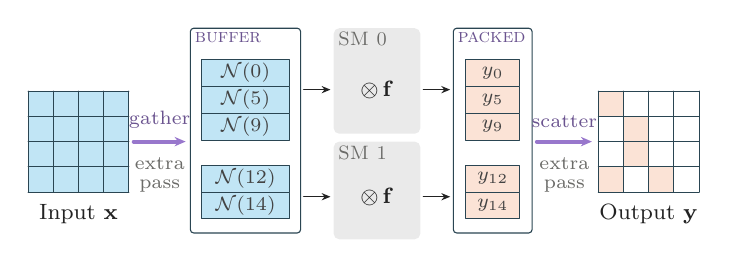
\begin{tikzpicture}[x=1mm, y=1mm]
  \def\s{3.2}   % grid cell
  \def\isact#1{\pgfmathparse{or(or(or(or(#1==0,#1==5),#1==9),#1==12),#1==14)}}
  \def\gy{-7.6} % top of the two grids
  \def\gm{\gy-2*\s}
  \def\rh{3.4}  % row height in the buffers
  % input x
  \fill[infill] (0, \gy) rectangle ++(4*\s, -4*\s);
  \foreach \k in {0,...,4} \draw[rule, line width=0.35pt] (\k*\s, \gy) -- ++(0, -4*\s) (0, \gy-\k*\s) -- ++(4*\s, 0);
  \node[title] at (2*\s, \gy-4*\s-1.2) {Input $\mathbf{x}$};
  % rows: SM 0 gets positions 0, 5, 9; SM 1 gets 12, 14
  \def\rowsA{-3.6/0, -7.0/5, -10.4/9}
  \def\rowsB{-17.0/12, -20.4/14}
  % gather buffer (memory)
  \def\bx{20.6}\def\bw{14.0}
  \draw[mem] (\bx, 0.4) rectangle ++(\bw, -26.0);
  \node[smlabel, text=gather!70!black] at (\bx, 0.4) {buffer};
  \foreach \yy/\p in {-3.6/0, -7.0/5, -10.4/9, -17.0/12, -20.4/14} {
    \fill[infill] (\bx+1.4, \yy) rectangle ++(\bw-2.8, -\rh);
    \draw[rule, line width=0.35pt] (\bx+1.4, \yy) rectangle ++(\bw-2.8, -\rh);
    \node[idx] at (\bx+\bw/2, \yy-\rh/2) {$\mathcal{N}(\p)$};}
  % SMs
  \def\cx{38.8}\def\cw{11.0}
  \fill[smfill, rounded corners=2pt] (\cx, 0.4) rectangle ++(\cw, -13.4);
  \fill[smfill, rounded corners=2pt] (\cx, -14.0) rectangle ++(\cw, -12.4);
  \node[smlabel] at (\cx, 0.4) {SM 0};
  \node[smlabel] at (\cx, -14.0) {SM 1};
  \node at (\cx+\cw/2, -7.4) {$\otimes\,\mathbf{f}$};
  \node at (\cx+\cw/2, -21.0) {$\otimes\,\mathbf{f}$};
  \draw[flow] (\bx+\bw+0.4, -7.4) -- (\cx-0.4, -7.4);
  \draw[flow] (\bx+\bw+0.4, -21.0) -- (\cx-0.4, -21.0);
  % packed outputs (memory)
  \def\ox{54.0}\def\ow{10.0}
  \draw[mem] (\ox, 0.4) rectangle ++(\ow, -26.0);
  \node[smlabel, text=gather!70!black] at (\ox, 0.4) {packed};
  \foreach \yy/\p in {-3.6/0, -7.0/5, -10.4/9, -17.0/12, -20.4/14} {
    \fill[actfill] (\ox+1.6, \yy) rectangle ++(\ow-3.2, -\rh);
    \draw[rule, line width=0.35pt] (\ox+1.6, \yy) rectangle ++(\ow-3.2, -\rh);
    \node[idx] at (\ox+\ow/2, \yy-\rh/2) {$y_{\p}$};}
  \draw[flow] (\cx+\cw+0.4, -7.4) -- (\ox-0.4, -7.4);
  \draw[flow] (\cx+\cw+0.4, -21.0) -- (\ox-0.4, -21.0);
  % output y: only the active positions are written
  \def\yx{72.4}
  \foreach \i in {0,...,15} {
    \pgfmathtruncatemacro\r{\i/4}\pgfmathtruncatemacro\q{mod(\i,4)}
    \isact{\i}
    \ifnum\pgfmathresult=1 \fill[actfill] (\yx+\q*\s, \gy-\r*\s) rectangle ++(\s, -\s); \fi
  }
  \foreach \k in {0,...,4} \draw[rule, line width=0.35pt] (\yx+\k*\s, \gy) -- ++(0, -4*\s) (\yx, \gy-\k*\s) -- ++(4*\s, 0);
  \node[title] at (\yx+2*\s, \gy-4*\s-1.2) {Output $\mathbf{y}$};
  % the two extra passes
  \draw[-{Stealth[length=4pt, width=3.4pt]}, line width=1.4pt, draw=gather] (13.4, \gm) -- (20.0, \gm);
  \node[anchor=south, text=gather!70!black, font=\fontsize{7}{7}\selectfont] at (16.7, \gm+0.5) {gather};
  \node[idx, text=muted, align=center, anchor=north] at (16.7, \gm-0.8) {extra\\pass};
  \draw[-{Stealth[length=4pt, width=3.4pt]}, line width=1.4pt, draw=gather] (64.6, \gm) -- (71.6, \gm);
  \node[anchor=south, text=gather!70!black, font=\fontsize{7}{7}\selectfont] at (68.1, \gm+0.5) {scatter};
  \node[idx, text=muted, align=center, anchor=north] at (68.1, \gm-0.8) {extra\\pass};
\end{tikzpicture}
\end{document}
